\documentclass[10pt,utf8]{beamer}

\mode<presentation> {
  \usetheme{Madrid}
  \setbeamercovered{transparent}
}

\usepackage{palatino}
\usepackage{graphicx}
\usepackage{array}
\usepackage{color}
\usepackage{subfigure}
\usepackage{colortbl}
\usepackage{amsmath}
\usepackage{hyperref}
\usepackage{listings}
\usepackage{pythonhighlight} % dnf install texlive-pythonhighlight

\setbeamertemplate{caption}{\raggedright\insertcaption\par} %turn off caption prefix ("Figure")

\definecolor{delim}{RGB}{20,105,176}
\definecolor{numb}{RGB}{106, 109, 32}
\definecolor{string}{rgb}{0.64,0.08,0.08}


\title{Kafka transactions and EOS}
\author{Vojtěch Juránek}
\institute[Red Hat]{Red Hat}
\date{May 24th 2024, Debezium F2F meeting, Brno}

\newenvironment{mylisting}
{\begin{list}{}{\setlength{\leftmargin}{1em}}\item\scriptsize\bfseries}
{\end{list}}

\newenvironment{mytinylisting}
{\begin{list}{}{\setlength{\leftmargin}{1em}}\item\tiny\bfseries}
{\end{list}}


\begin{document}

%\tikzstyle{every picture}+=[remember picture]
%\tikzstyle{na} = [baseline=-.5ex]


\begin{frame}
    \titlepage
\end{frame}

\begin{frame}
    \frametitle{Kafka transactions}
    \begin{itemize}
        \item Atomic writes across multiple Kafka topics and partitions.
        \item Atomic read-process-write cycles.
        \item Consumer delivers transactional messages to the application only if the transaction was committed.
        \item However, consumer is not guaranteed to be subscribed to all partitions that are part of the transaction.
    \end{itemize}
\end{frame}

\begin{frame}
    \frametitle{Kafka transactions}
    \begin{figure}
        \centering
        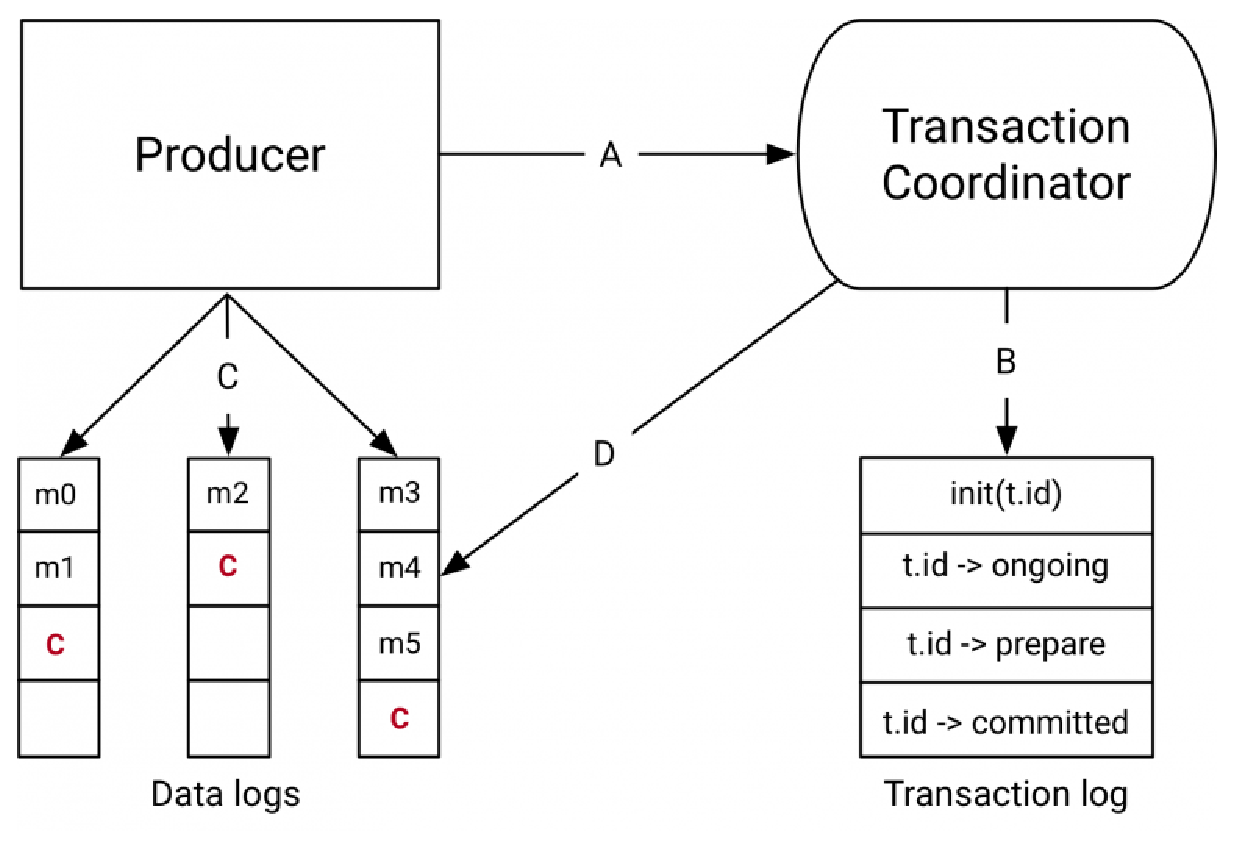
\includegraphics[height=6cm]{./img/kafka_transactions.eps}
        \caption{\tiny{Source: \url{https://www.confluent.io/blog/transactions-apache-kafka/}}}
    \end{figure}
\end{frame}


\begin{frame}
    \begin{itemize}
        \item Each producer has to define \texttt{transactional.id}
        \begin{itemize}
            \item identifies producer across restarts
            \item used for zombie fencing - each \texttt{transactional.id} has associate \texttt{epoch} number which increases after (re)start
        \end{itemize}
    \end{itemize}
\end{frame}

\begin{frame}
    \frametitle{Kafka transactions configuration}
    Producer config:
    \begin{itemize}
        \item \texttt{enable.idempotence=true}
        \item \texttt{transactional.id=12345}
    \end{itemize}
    \vspace{0.5cm}
    Consumer config:
    \begin{itemize}
     \item \texttt{isolation.level=read\_uncommitted|read\_committed}
    \end{itemize}
    \vspace{0.5cm}
    Broker config - has the sane defaults
\end{frame}

\begin{frame}
    \frametitle{Resource}
    \begin{itemize}
        \color{blue}
        \item \href{https://cwiki.apache.org/confluence/display/KAFKA/KIP-98+-+Exactly+Once+Delivery+and+Transactional+Messaging}{Kafka KIP-98: Exactly Once Delivery and Transactional Messaging}
        \item \href{https://docs.google.com/document/d/11Jqy\_GjUGtdXJK94XGsEIK7CP1SnQGdp2eF0wSw9ra8/edit\#heading=h.xq0ee1vnpz4o}{Exactly Once Delivery and Transactional Messaging in Kafka (design document)}
        \item \href{https://www.confluent.io/blog/transactions-apache-kafka/}{Transactions in Apache Kafka (Confluent blog)}
        \item \href{https://cwiki.apache.org/confluence/display/KAFKA/KIP-618\%3A+Exactly-Once+Support+for+Source+Connectors}{Kafka KIP-618: Exactly-Once Support for Source Connectors}
        \item \href{https://strimzi.io/blog/2023/05/03/kafka-transactions/}{Exactly-once semantics with Kafka transactions (Strimzi blog)}
        \color{black}
    \end{itemize}
\end{frame}


%%%%%%%%%%%%%%%%%%%%%%%%%%%%%%%%%%%%%%%%%%%%%%%%%%%%%%%%%%%%%%%%%%%%%%%%%%%%%%%%%%%%%%%%%%%%%%%%%
%%% BACKUP
%%%%%%%%%%%%%%%%%%%%%%%%%%%%%%%%%%%%%%%%%%%%%%%%%%%%%%%%%%%%%%%%%%%%%%%%%%%%%%%%%%%%%%%%%%%%%%%%%

% \begin{frame}
%     \centering
%     \huge{\textbf{Backup slides}}
% \end{frame}

\end{document}
